\documentclass{standalone}
\usepackage{tikz}
\usepackage{ctex,siunitx}
\usepackage{tkz-euclide}
\usepackage{amsmath}
\usetikzlibrary{patterns, calc}
\usetikzlibrary {decorations.pathmorphing, decorations.pathreplacing, decorations.shapes,}
\begin{document}
\small
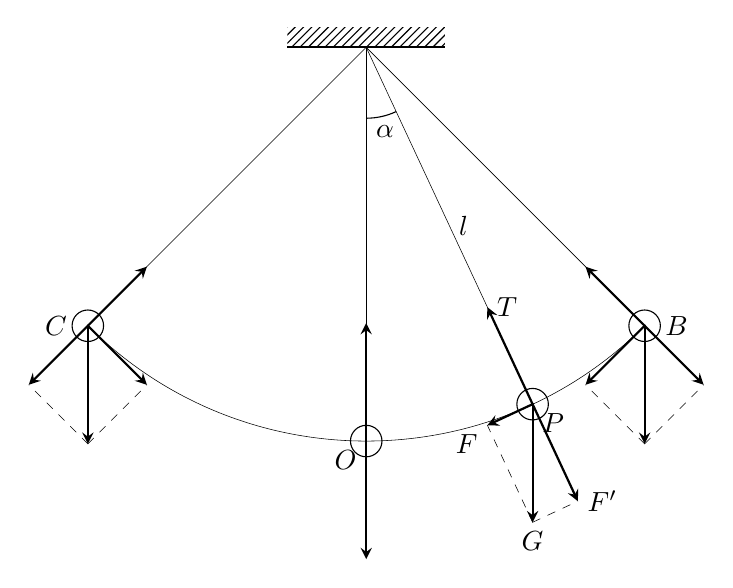
\begin{tikzpicture}[>=stealth]
  \fill[pattern=north east lines](-1,0) rectangle (1,.25);
  \draw[thick](-1,0)--(1,0);
  \tkzDefPoints{0/0/O', 0/-5/O, 0/-6.5/G}
  \tkzDefPoint(-135:5){C}
  \tkzDefPoint(-65:5){P}
  \tkzDefPoint(-45:5){B}
  \tkzDrawSegments(O',B O',O O',C O',P)
  \tkzDefPointsBy[translation = from O to G](B,C,P){G1,G2,G3}
  \tkzDrawSegments[thick,->](O,G B,G1 C,G2 P,G3)
  \tkzDrawArc(O',C)(B)
  \foreach \x in {O,B,C,P}
  {
      \draw(\x) circle(.2);
  }
  \foreach \x/\y in {B/G1,C/G2,P/G3}
  {
      \tkzDefPointBy[projection = onto O'--\x](\y)
      \tkzGetPoint{\x'}
      \tkzDefPointsBy[translation= from \x' to \x](\y){\x''}
      \tkzDrawSegments[thick, ->](\x,\x'' \x,\x')
      \tkzDrawSegments[dashed](\y,\x' \y,\x'')
  }
  \tkzLabelPoint[below left](P''){$F$}
  
  \foreach \x/\y in {B/B', C/C', O/G, P/P'}
  {
      \tkzDefPointBy[symmetry=center \x](\y)
      \tkzGetPoint{\y'}
      \tkzDrawSegments[thick, ->](\x,\y')
  }
  \tkzLabelPoints[left=4pt](C)
  \tkzLabelPoints[below left](O)
  \tkzLabelPoints[below right](P)
  \tkzLabelPoints[right=4pt](B)
  \tkzMarkAngles[mark=none, size=.9](O,O',P)
  \tkzLabelAngle[pos=1.1](O,O',P){$\alpha$}
  \tkzLabelSegment[right](O',P){$l$}
  \tkzLabelPoint[below](G3){$G$}
  \tkzLabelPoint[right](P'){$F'$}
  \tkzLabelPoint[right](P''){$T$}
\end{tikzpicture}
\end{document}